
% C.H. Re-write of this section!

\begin{summary}
Co-I Hirata is leading the development of the HLS observing plan, extending his
previous tools used for the SDT. These tools incorporate observing constraints
in the chosen orbit, an exposure-by-exposure observing sequence optimized with
detailed model of overheads, and tiling/coverage maps including field
distortions and curved sky effects. These tools treat both imaging and
spectroscopy with unified functions and scripts, and are well suited to joint
survey optimization when both hardware parameters (e.g., reaction wheel
orientations) and the observing program (e.g., depth vs.\ area) are considered.
This effort is coordinated with the scheduling and Design Reference Mission (DRM)
Working Groups. We are both providing an example detailed plan for the HLS to
the DRM working group, and cross-checking the Project's spreadsheet-level survey
calculators against our simulations. The HLS observing plan is also being
transferred to the Calibration Working Group, since the HLS observing strategy
feeds directly into the issue of self-calibration.
\end{summary}

\subsection{Survey Optimization Principles}
%==========================================
%\Auth{David W, Chris, Olivier}
\label{sec:sur_opt}

%%%%The key constraint in survey optimization is the limited amount of observational time
%%%%available, since WFIRST is life-time limited and has multiple science focus areas.
%%%%For fixed instrumental capabilities and observing time, the most basic
%%%%decision to make about survey strategy is the trade between depth and total area.
%%%%In optimizing the WFIRST WL and BAO/RSD surveys, there are two key considerations:
%%%%(i) {\em precision} -- to maximize the DE science return of WFIRST, taking advantage of synergy with other surveys; and
%%%%(ii) {\em accuracy} -- tight control of systematic uncertainties, to ensure correct DE measurements.
The key constraint in survey optimization is the limited amount of observational time
available, since WFIRST is life-time limited and has multiple science focus areas.
For fixed instrumental capabilities and observing time, the primary
decisions on survey strategy are the trade between depth and total area, and
the balance between imaging and spectroscopy.
These decisions are driven by two major considerations:
\begin{itemize}
\item \emph{Pecision} -- to maximize the DE science return of WFIRST, taking advantage of synergies with other surveys; and
\item \emph{Accuracy} -- tight control of systematic uncertainties, to ensure correct DE measurements.
\end{itemize}
The combined expertise of our team in WL and GRS enables us to rapidly evaluate
these trades.

\paragraph{HLIS} The statistical power of a WL survey scales with the
total number of galaxy shape measurements, the product of the survey area and the effective surface density.
The SDT2015 report adopts an HLS imaging exposure time that yields roughly equal
contributions from read noise and sky noise in the most sensitive
filters, which approximately maximizes the total number of shape
measurements. This is a compromise between minimizing overheads and
read noise (which favors a ``deep'' mode), versus the shallow number
counts of resolved WL sources (shallower than $N\propto F^{-2}$, which
favors a ``wide'' mode). We re-examined the depth vs.\ area trade using
higher-fidelity tools (e.g., incorporation of shape measurement noise from realistic simulations, and updated
detector properties) and propagating the trades all the way to cosmological parameters
(using \CoLi).

\paragraph{HLSS} The depth vs.\ area trade for the GRS is driven by two
competing factors: for deep surveys, where the number density of galaxies $n$ is
large ($nP\gg 1$, where $P$ is the power spectrum at a given scale), the
information per unit area saturates; whereas for wide surveys, overheads reduce
inefficiency and galaxy shot noise inflates the statistical errors. In the SDT15
survey design, the GRS covers the same area as the HLS imaging survey ($\approx
2,200\deg^2$), to a $7\sigma$ limiting line flux of $\sim 10^{-16}
\erg\cm^{-2}\,{\rm s}^{-1}$ over most of the grism bandpass. This yields
approximately the largest number of galaxy redshifts for a fixed total observing
time. SDT15 found that doubling the survey area at fixed observing time (even
without additional imaging) {\it reduces} the precision of BAO measurements
because of the rapid increase in galaxy shot noise with decreasing spectroscopic
depth. However, this conclusion is sensitive to the luminosity function of
H$\alpha$ emitters at $z=1-2$, which remains uncertain
\cite{Mehta:2015,Pozzetti:2016}; Co-Is Teplitz and Wang lead our efforts to
reduce this uncertainty and feed the results into optimization of the GRS
(\S~\ref{sec:LF}).


\subsection{Snapshot of the HLS observing plan}
\label{ss:snapshot}

\begin{summaryii}
Our team provided a ``snapshot'' of the HLS observing sequence to the full FSWG
on April 19, 2017. This is by no means a final or even optimized version of the
HLS, but is a work in progress as a result of trades in Phase A, as well as the
recent decision to reduce the primary mission to 5 years.
\end{summaryii}

Major updates relative to the SDT plan have included:
\begin{itemize}
\item A Lissajous orbit around L2. This is presently a place-holder, as the exact orbit has not yet been selected (and would depend on the launch date), but it gives a possible sampling of Sun, Earth, and Moon constraints.
\item A rotated WFI (by 90$^\circ$ relative to the Cycle 6 design).
\item Recommended slew and settle times provided by the Project.
\item Faster detector readout (200 kHz instead of 100 kHz).
\item Changes to the exposure time and dithering strategy to accommodate a
5-year baseline mission (as is to be presented to the WIETR). Specifically, we
reduced exposure time to 140.2 s (imaging) and 297.0 s (spectroscopy); and
changed the dither pattern in J band. (We are working on checking this strategy
with image simulations, if it causes a problem we may have to revert.)
\item Implemented bright star avoidance (observations are skipped if there is an $H_{\rm AB}\le 3$ star within 6 arcmin of any SCA).
\end{itemize}
Known current issues with the snapshot plan include:
\begin{itemize}
\item
The SN and coronagraph programs in the code haven't been updated since the SDT
(except to cut the mission time by a factor of 5/6), even though they will
likely change significantly. As in the SDT report, the coronagraph has blocks of
time reserved. This will evolve in order to align the HLS plan with the other
groups, as well as any changes to the scheduling architecture that we are
directed to implement (e.g.\ block scheduling).
\item
We have begun putting the deep fields into this document, but right now they are
(i) not fully specified, (ii) the tiling is not optimized, and (iii) some roll
angles don't align with WFIRST constraints (hence didn't schedule). These issues
will be solved in the next snapshot.
\end{itemize}

We note that \emph{no policy decisions should be inferred from this sequence},
as these will come from a higher level.

The survey bounding box is 2,097 deg$^2$. The area covered with $\ge 3$ exposures
in every filter and the grism, including edge effects and holes around the
bright stars, is 1,947 deg$^2$. The time required for this version of the HLS is
394 days (imaging) + 215 days (spectroscopy).

The scheduling tools output a set of charts, included in this package:
\begin{itemize}
\item
Fig.~\ref{fig:observing_chart}: Graphical display of the 5-year observing sequence.
\item
Fig.~\ref{fig:hls_depth}: HLS distribution of number of exposures in each filter.
\item
Fig.~\ref{fig:hls_dust}: HLS distribution of dust column [$E(B-V)$ in magnitudes]. Cosmological forecasts are based on a dust column of $E(B-V)=0.035$ mag.
\item
Fig.~\ref{fig:hls_bright}: HLS distribution of zodiacal light (normalized to 1 at the ecliptic poles averaged over the year). Cosmological forecasts are based on a zodiacal brightness of 1.60 (except for 1.75 in the F184 filter, which is the least sensitive to zodiacal light and therefore was scheduled at inferior times of year).
\item
Fig.~\ref{fig:footprint}: The footprint of the HLS on the sky. This is an area of ongoing optimization, as we consider the needs of the deep fields, overlap with LSST, and the fraction of the survey footprint accessible from Northern observatories such as Subaru.
\end{itemize}

\begin{figure}
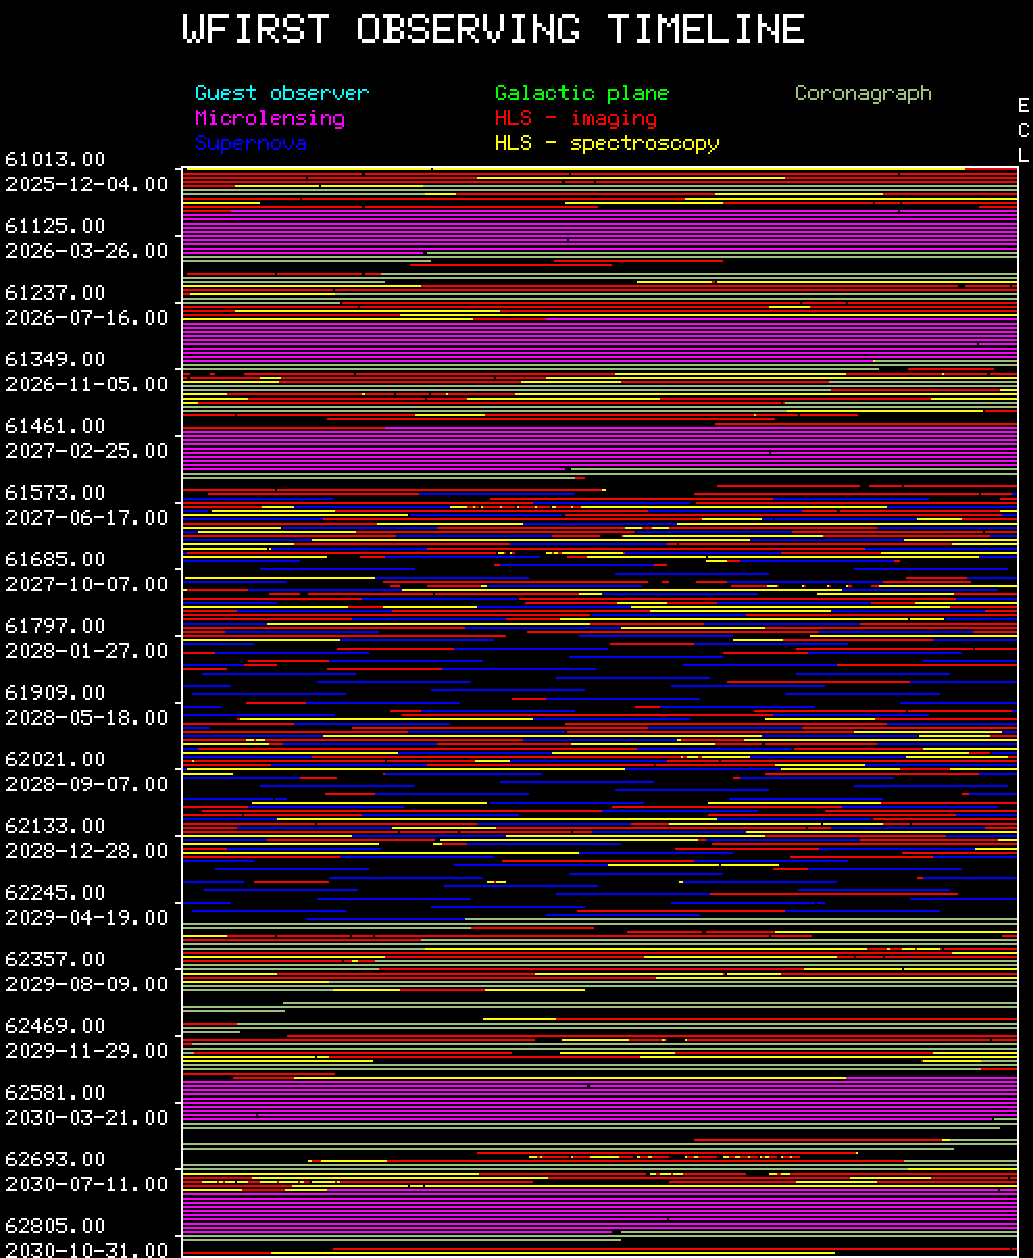
\includegraphics[height=8in]{Plots/observing_chart.pdf}
\caption{\label{fig:observing_chart}Observing timeline. Each row represents 7 days of observations, and is color-coded according to the observing program. Note the microlensing seasons (magenta), supernova survey (blue: $\sim$5-day cadence), and HLS (red+yellow). Blank areas are not allocated. Labels on the left-hand side are shown every 16 weeks.}
\end{figure}

\begin{figure}
\includegraphics[width=5in]{Plots/hlsdepth.pdf}
\caption{\label{fig:hls_depth}The cumulative distribution of HLS exposure depths above a certain area. The pile-up with many exposures at small area is the result of the deep fields.}
\end{figure}

\begin{figure}
\includegraphics[width=5in]{Plots/hlsdust.pdf}
\caption{\label{fig:hls_dust}The cumulative distribution of Galactic dust in the HLS.}
\end{figure}

\begin{figure}
\includegraphics[width=5in]{Plots/hlsbright.pdf}
\caption{\label{fig:hls_bright}The cumulative distribution of zodiacal light in the HLS.}
\end{figure}

\begin{figure}
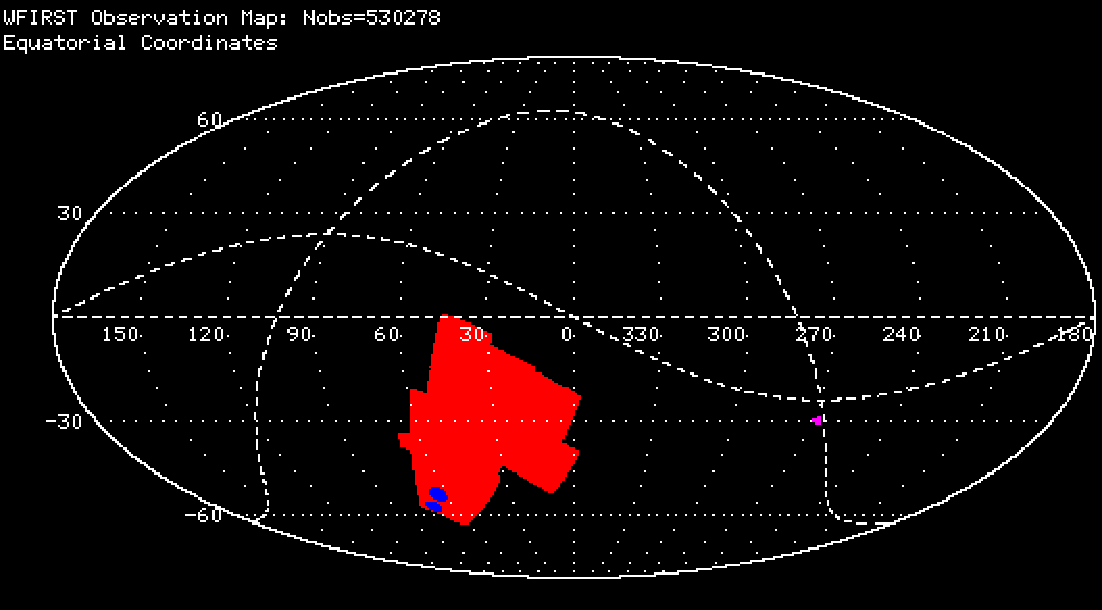
\includegraphics[width=6in]{Plots/sky-equ.pdf}
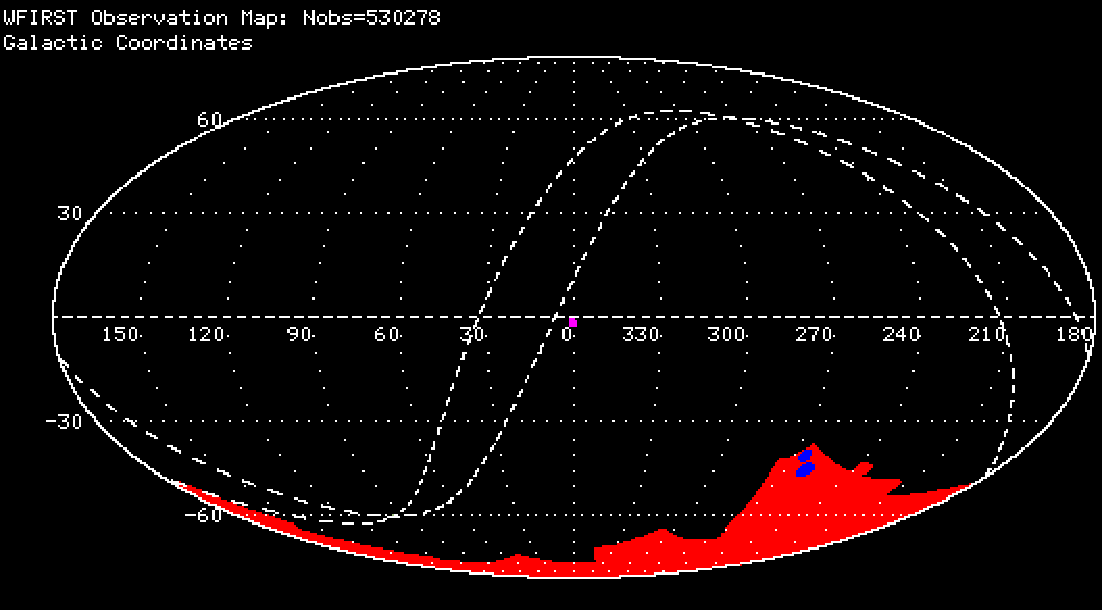
\includegraphics[width=6in]{Plots/sky-gal.pdf}
\caption{\label{fig:footprint}The footprint of the HLS (red) in Equatorial (top) and Galactic (bottom) coordinates.}
\end{figure}

\subsection{Further optimizations}

\begin{summaryii}
Our team plans to study further optimizations to the HLS -- including more
drastic changes such as multi-tiered surveys, or a significant re-balancing of
area vs.\ depth -- in Phase B. However, in preparation for SRR/MDR, our main
focus has been on demonstrating at least one survey configuration that meets
requirements, and the construction of tools that link the observing strategy to
calibration studies (\S\ref{sec:wl_calibration}) and image simulations (\S\ref{sec:hlis_image_sim}).
\end{summaryii}

The optimization of the WFIRST HLS will be tightly linked to operations simulations,
which inform the possible range of footprint area and location, depth in each filter (or grism), redundancy,
and temporal distribution of exposures. We propose a highly integrated approach, with the
operations simulations at the core, but with links to pixel-level simulations to assess required
redundancy, cosmological forecasting tools (\CoLi) to assess science reach, and comparison to the
observing regions of other surveys and telescopes to maximize synergies and meet requirements for
deep fields and photo-$z$ calibration.

% I hope this figure will just be combined with Fig 1.

%
%\setlength\intextsep{-2pt}
%%\begin{center}
%\begin{wrapfigure}{!ht}{0.45\textwidth}
% \begin{boxedminipage}{0.45\textwidth}
% \begin{center}
%\includegraphics[width=1.0\textwidth]{plots/like_DES_WFIRST_combi.eps}
% \end{center}
% \vspace{-1.25cm}
%\caption{{\footnotesize{ \Oli{Initial version for WFIRST vs DES} forecasts multi-probe science case. Probes included are cosmic shear, galaxy clustering, and galaxy-galaxy-lensing from WFIRST (black) in comparison to the Dark Energy Survey (green). The analysis includes BAO, SN1a and Planck information and accounts for galaxy bias, shear calibration, and photo-z errors (with different assumptions for the weak lensing and for the clustering sample). }}}
% \label{tab:milestones}
%\end{boxedminipage}
%\end{wrapfigure}
%% \end{center}
%\setlength\intextsep{0pt}

% \setlength\intextsep{-2pt}
% \begin{wrapfigure}{!ht}{0.75\textwidth}
%  \begin{boxedminipage}{0.75\textwidth}
%  \begin{center}
% \begin{figure*}
% \includegraphics[width=0.5\textwidth]{plots/WFIRST_multi.eps}
%% \caption{\textit{Placeholder plot for WFIRST forecasts multi-probe science case. Probes included are cosmic shear, galaxy clustering, and galaxy-galaxy-lensing, BAO with and without systematics (black and red contours, respectively). The systematics considered in this analysis are shear and photo-z uncertainties (which have different assumptions for the weak lensing and for the clustering sample), and linear galaxy bias. Blue contours include information from DES supernovae type 1a and green contours include an approximate version of Planck CMB temperature and polarization information.}}
%% {\bfseries C.H.: This belongs in another section.}
%%          \label{fi:WFIRST_multi1}
%% \end{figure*}

\subsection{Operations model (D7)}

Co-I Hirata will lead the development of the HLS observing plan,
extending his previous tools used for the SDT. These tools are already
highly advanced, incorporating observing constraints in the candidate
orbits (Geostationary Earth Orbit (GEO) or at the Lagrange point L2),
an exposure-by-exposure observing sequence optimized
with detailed model of overheads, and tiling/coverage maps including
field distortions and curved sky effects. These tools treat both imaging
and spectroscopy with unified functions and scripts, and are well suited to joint survey optimization when
both hardware parameters (e.g., reaction wheel orientations) and the
observing program (e.g., depth vs.\ area) are considered.
Hirata's operations tools were
used by the SDT for ``proof of principle'' studies, but we will now
extend them to (i) evaluate survey performance at intermediate stages
(e.g., what information is available after 1, 2, or 4 years); (ii)
include a pilot survey in the first few months of the mission to
validate HLS performance and make any ``early changes'' necessary;
(iii) include dedicated calibration observations as needed; and (iv)
export field overlap statistics as needed to assess internal calibration
strategies such as ``uber-calibration'' \cite{Padmanabhan2008}. This work will
be performed in consultation with other science groups on the FSWG and with
the WSC.

The SDT coverage maps included a study of the overlap with the LSST footprint,
but with our links to other projects we will understand the overlap with
the other cosmology surveys as well as the accessibility
of our fields from ground-based telescopes. This information, combined with the
community workshops (\S\ref{sec:engagement}), will be used to maximize synergies with
other facilities as well as ensure that potentially conflicting requirements (e.g.,
overlapping LSST photometry and photo-$z$ calibration including Northern telescopes
such as Subaru or Keck) can be met.

%\subsection{Synergies of WFIRST internal probes}
%=====================

%\subsection{Synergies of WFIRST and external data sets}
%=====================

\subsection{Survey Optimization (D10, D11)}
%=================================================
%\Auth{David W, Chris, Olivier}
\label{sec:sur_opt}

%%%%The key constraint in survey optimization is the limited amount of observational time
%%%%available, since WFIRST is life-time limited and has multiple science focus areas.
%%%%For fixed instrumental capabilities and observing time, the most basic
%%%%decision to make about survey strategy is the trade between depth and total area.
%%%%In optimizing the WFIRST WL and BAO/RSD surveys, there are two key considerations:
%%%%(i) {\em precision} -- to maximize the DE science return of WFIRST, taking advantage of synergy with other surveys; and
%%%%(ii) {\em accuracy} -- tight control of systematic uncertainties, to ensure correct DE measurements.
The key constraint in survey optimization is the limited amount of observational time
available, since WFIRST is life-time limited and has multiple science focus areas.
For fixed instrumental capabilities and observing time, the primary
decisions on survey strategy are the trade between depth and total area, and
the balance between imaging and spectroscopy.
These decisions are driven by two major considerations:
(i) {\em precision} -- to maximize the DE science return of WFIRST, taking advantage of synergies with other surveys; and
(ii) {\em accuracy} -- tight control of systematic uncertainties, to ensure correct DE measurements.
The combined expertise of our team in WL and GRS will enable us to rapidly evaluate
these trades, informed by results from previous and concurrent surveys such as
DES/DESI/Euclid. Furthermore, we plan on developing pipelines to
rapidly analyse ``pilot'' data from WFIRST to quantify the telescope
and instrument performance, as well as developing well defined metrics to guide the survey trades.

\subs{WL Survey.} The statistical power of a WL survey scales with the
total number of galaxy shape measurements, the product of the survey area and the effective surface density.
The SDT2015 report adopts an HLS imaging exposure time that yields roughly equal
contributions from read noise and sky noise in the most sensitive
filters, which approximately maximizes the total number of shape
measurements. This is a compromise between minimizing overheads and
read noise (which favors a ``deep'' mode), versus the shallow number
counts of resolved WL sources (shallower than $N\propto F^{-2}$, which
favors a ``wide'' mode). However, we will re-examine the depth vs.\ area trade using
higher-fidelity tools (e.g., incorporation of shape measurement noise from realistic simulations, and updated
detector properties) and propagating the trades all the way to cosmological parameters
(using \CoLi).
We will also investigate the performance of hybrid strategies in
which a four-filter survey over part of the HLS area is combined
with a one- or two-filter survey over a larger area.  This approach
would yield more independent shape measurements at the cost of
greater \photoz\ uncertainties and complicating cross-checks of systematics,
so assessing it requires attention to the entire path from data
to scientific conclusions, including the impacts
on scientific investigations outside of dark energy and cosmological
parameters.

\subs{GRS Survey.} The depth vs.\ area trade for the GRS is driven
by two competing factors: for deep
surveys, where the number density of galaxies $n$ is large ($nP\gg 1$, where $P$ is the power spectrum at
a given scale), the information per unit area saturates; whereas for wide surveys, overheads
reduce inefficiency and galaxy shot noise inflates the statistical errors.
In the SDT15 survey design,
the GRS covers the same area as the HLS imaging survey
($\approx 2,200\deg^2$), to a
$7\sigma$ limiting line flux of $\sim 10^{-16} \erg\cm^{-2}\,{\rm s}^{-1}$
over most of the grism bandpass.
This yields approximately the largest number of galaxy
redshifts for a fixed total observing time.
SDT15 found that doubling the survey area at fixed observing time (even without
additional imaging) {\it reduces} the precision of BAO measurements
because of the rapid increase in galaxy shot noise with decreasing
spectroscopic depth.
However, this conclusion is sensitive to the luminosity function of
H$\alpha$ emitters at $z=1-2$, which remains uncertain \cite{Mehta:2015,Pozzetti:2016};
Co-Is Teplitz and Wang will lead our efforts to reduce this uncertainty
and feed the results into optimization of the GRS.

We will study the link between the observing strategy and systematic error
validation.  For example, pixel-level simulations will predict the variation of
galaxy density with respect to the diversity of roll angles, use of subsets of
the exposures in the data reduction, etc.; our team has extensive experience
with the measurement of such dependences in imaging surveys (Co-Is Ho, Hirata,
Padmanabhan)
and will extend this to the GRS. The hardest part of the GRS error
validation will be galaxy biasing: while it is possible to ``test'' bias models
against a range of simulations with plausible prescriptions for galaxy
placements (HODs, SAMs, etc.), we will ultimately need to validate galaxy
biasing models against the data itself. The most promising avenues are
higher-order statistics (such as 3-point correlations)
and the consistency of results obtained from subsets of the galaxy sample
(e.g., split by magnitude or color).
Both of these demand larger $nP$ and drive
the survey deeper than the power spectrum measurement.
We will develop the tools to assess the precision of these
validation tests and will incorporate them into the survey optimization.

A key consideration in the depth vs.\ area trade is the relation to the Euclid
and DESI redshift surveys; the optimization of WFIRST GRS should avoid portions
of this space that will already be well-explored by these other projects and
focus on the unique capabilities provided by a large telescope in the
low-background space environment.

%Given the assumptions about instrument
%performance and empirical model of the H$\alpha$ luminosity function
%adopted in SDT2015, this exposure time is approximately the one that
%yields the largest number of galaxy redshifts for a fixed total
%In the SDT2015
%survey design, the GRS covers the same area as the HLS imaging survey
%($\approx 2200\deg^2$), and the exposure time of 347 sec yields a
%$7\sigma$ limiting line flux of $\approx 10^{-16} \erg\cm^{-2}\sec^{-1}$
%over most of the grism bandpass.
%
%observing time (0.68 years in SDT2015).
%However, the statistical power
%of a redshift survey does not scale trivially with the number of galaxies,
%and the optimal choice can be quite different for different applications.
%
%The variance in a measurement of the galaxy power spectrum at
%wavenumber $k$ scales inversely with the effective comoving survey volume
%\begin{equation}
%V_{\rm eff}(k) = \int d^3r  [1+nP(k)]^{-1}~,
%\end{equation}
%where $n$ is the galaxy space density.  {\bf Agreed?}
%The optimal tradeoff between depth and area typically occurs
%for $nP = 1-2$; at higher $nP$ it is better to expand the survey
%area to increase volume, while at lower $nP$ it is better to
%go deeper to reduce shot noise.
%SDT2015 forecasts $nP \approx 2-3$ (depending on redshift)
%at the scale $k=0.2\mhmpcinv$
%that is relevant for BAO precision, which suggests that the BAO
%precision could be improved moderately by decreasing the exposure
%time and increasing the survey area; because the survey depth is
%already on the exponential tail of the H$\alpha$ luminosity function,
%the space density drops rapidly with increasing flux limit.
%However, even for the relatively simple case of BAO, optimization
%depends sensitively on instrument characteristics (detector read noise,
%grism throughput, etc.), on the imperfectly known H$\alpha$ and [OIII]
%luminosity functions, on the performance of reconstruction methods,
%and on details of data reduction and incompleteness corrections.
%For example, the methods recently proposed by \cite{suchyta2015}
%could allow effective use of emission line sources down to a $\sim 5\sigma$
%limit, instead of the conservative $7\sigma$ detection threshold assumed by
%SDT2015, and this would significantly shift the optimal exposure time.
%For RSD the optimization depends additionally on the accuracy of theoretical
%techniques to model non-linear galaxy clustering, since this determines
%the maximum wavenumber at which power spectrum measurements are cosmologically
%useful.  We also hope that the methodology investigations described
%above will provide powerful new routes to cosmological parameter constraints
%from higher order clustering measurements, which are more sensitive to
%shot noise.  Relative to power spectrum analyses, these methods likely
%favor a denser survey with higher $nP$, but survey optimization for
%such analyses is largely uncharted territory.

\subs{WFIRST HLS Survey.}  Optimization of the WFIRST HLS requires the end-to-end approach
outlined in this proposal, considering everything from the read noise
of the detectors and contamination of redshift catalogs to the
theoretical modeling systematics for higher order clustering statistics.
It also requires joint consideration of the imaging and spectroscopic
surveys:
multi-filter photometry (as planned in SDT2015) is required to suppress
contaminants in the GRS \cite{Pullen2015}.
We will provide, in addition to our own recommendations,
publicly available tools that can be used by future science teams,
the WFIRST Project, and the community at large to evaluate a variety
of HLS strategies, including changes to the balance between imaging
and spectroscopy.  These tools will enable us and others to incorporate
updated information about instrument and software performance,
empirical data on the galaxy population, progress in modeling techniques,
the expected contributions of other projects like DESI, LSST, and Euclid,
and changes in the experimental dark energy landscape that highlight
the importance of particular classes of measurements.

%}
